% Section OOA
% Objekt Orientierte Analyse

\section{OOA}

\subsection{Ziel der Analyse}
  \begin{itemize}[leftmargin = 0.5cm]
    \item Wünsche und Anforderungen an  ein neues System ermitteln und beschreiben
    \item Bei Modellbildung bewusst \textbf{alle} Aspekte der Implementierung ausklammern
    \item System als ideal anschauen. D.h keine Verzögerungen, keine Fehler, unendlicher Speicher
  \end{itemize}
  
\subsection{Ziel der OOA}
  Ziel ist es, das zu realisierende Problem zu verstehen und in einem OOA-Modell zu beschreiben.
  
\subsection{OOA Modelle}
  \begin{description}
    \item[statisches Modell] 
      beschreibt $\ldots$
      \begin{description}[leftmargin=0.5cm]
        \item[$\ldots$] die Klassen des Systems
        \item[$\ldots$] die Assoziation zwischen den Klassen
        \item[$\ldots$] die Generalisierung (Vererbung)
      \end{description}
      ausserdem enthält es die Daten des Systems (Attribute)
     
    \item[dynamisches Modell]
      \begin{itemize}[leftmargin=0.5cm]
        \item zeigt die Funktionsabläufe
        \item Use-Cases beschreiben die durchzuführenden Aufgaben
        \item Aktivität beschreibt die Ausführung von Funktionalität und Verhalten
        \item Szenario zeigen wie Objekte miteinander kommunizieren
        \item Zustandsautomaten beschreiben in der Analyse die Reaktion eines Objektes auf verschiedne Ereignisse
      \end{itemize}
      
    \item[OOA-Modell]
      \begin{itemize}[leftmargin=0.5cm]
        \item beschreibt die essenzielle Struktur und Semantik des Problems, aber noch keine technische Beschreibung
        \item enthält keinerlei Optimierung für das verwendete Computersystem oder die benutzte Basissoftware
        \item bildet fachliche Lösung des zu realisierenden Systems
      \end{itemize}
      
    \item[primitive Datentypen]
      \begin{itemize}[leftmargin=0.5cm]
        \item Boolean
        \item String
        \item Integer
        \item UnlimitedNatural
      \end{itemize}
  \end{description}
  
\subsection{Attribut \balzert{26}}
  \begin{description}
    \item[Attribut] 
      Beschreibt Daten die von den Objekten der Klasse angenommen
      werden können. Alle Objekte einer Klasse haben dieselben Attribute, können
      aber unterschiedliche Attributwerte haben.
    \item[Klassenattribut] 
      Wenn nur ein Attributwert für alle Objekte einer Klasse existiert. 
      Sie existieren auch, wenn es zu einer Klasse noch keine Objekte gibt.
      Wird \underline{unterstrichen}
    \item[abgeleitets Attribut]
      kann zu jeder Zeit aus anderen Attributwerten berechnet werden. Wird mit \textbf{/zahl} geschrieben.  
    \item[Eigenschaftswerte]
      siehe \Balzert{29}      
    \item[Multiplizität]
      [0..n] $\rightarrow$ spezifiziert, [0..*] $\rightarrow$ unspezifiziert
  \end{description}
  
\subsection{Klasse \balzert{23}}
  Eine Klasse ist eine Vorlage für ein Objekt.\\
 \begin{minipage}[t]{4cm}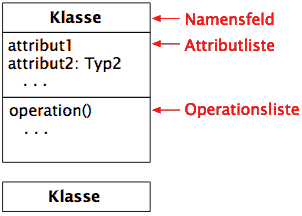
\includegraphics[width=4cm]{./bilder/klasse}\end{minipage}
 \begin{minipage}{15cm}
   \begin{description}
    \item[Operation] 
      Eine Funktion die auf alle Attributwere eines Objekts Zugriff hat.
    \item[Klassenoperation] 
      Eine Operation, die der jeweiligen Klasse zugeordnet ist. 
      Kann nicht auf 
      ein einzelnes Objekt der Klasse angewendet werden. Wird \underline{unterstrichen}
    \item[Verhalten] 
      Das Verhalten der Klasse ist die Menge aller Operationen
    \item[Abstrakte] 
      Von einer abstrakten Klasse können keine Objekte erzeugt werden. 
      (\textit{kursiver Klassenname} oder $\lbrace$abstract$\rbrace$)
    \item[Basisklasse] 
      Vererbt abgeleiteten Klassen Attribute und Operationen
  \end{description}
  \end{minipage}
  
  \subsubsection{Notation}
  		Der \textbf{Klassenname} ist immer ein Substantiv im Singular, das durch ein Adjektiv
  		ergänzt werden kann. Der Klassenname wird fett geschrieben und beginnt mit einem
  		Grossbuchstaben. \\
  
\subsection{Objekt \balzert{20}}
	Ein Objekt wird aus einer Klasse erzeugt, ist also ein Exemplar einer Klasse.
	\begin{description}
		\item[Zustand] 
      Bestimmt durch seine Attributwerte und seine Objektbeziehungen zu anderen Objekten
		\item[Verhalten] 
      Die beobachtbaren Effekte aller Operationen bestimmt durch die Operationsaufruf, 
      auf die diese Klasse bzw. deren Objekte reagieren.
		\item[Objektidentität] 
      jedes Objekt hat eine Identität, welche einzigartig ist (unique)
	\end{description}
	
	\subsubsection{Notation}
			Objektnamen werden immer klein geschrieben und unterstrichen. \\
		\begin{tabular}{l l}
			\underline{:Klasse} & anonymes Objekt \\
			\underline{objekt:Klasse} & Objekt wird über Namen angesprochen \\
			\underline{objekt} & wenn Objektname zur Identifikation ausreicht \\
		\end{tabular}\\
		
	\begin{multicols}{2}	
		\subsubsection{Geheimnisprinzip}
		Daten sind nach aussen verborgen und können nur über Operationen gelesen oder geändert werden.\\
		\subsubsection{Objektidentität}
		Eigenschaft, die ein Objekt von allen anderen Objekten unterscheidet. Bei zwei Objekten
		mit gleichen Attributwerten sprechen wir von Gleichheit, wenn dasselbe Objekt gemeint
		ist von Identität.
	\end{multicols}
	
  
\subsection{Assoziation \balzert{42}}
	Modelliert Objektbeziehungen zwischen Objekten einer oder mehrerer Klassen.
	Jede Assoziation wird durch Mutliplizitäten, einen optionalen Namen oder Rollennamen
	beschrieben.
  \begin{description}
    \item[binäre Assoziation] 
      Assoziation zwischen 2 Objekten
    \item[ternäre Assoziation] 
      Assoziation zwischen 3 Objekten
    \item[n-äre Assoziation] 
      zwischen n Objekten
    \item[reflexive Assoziation] 
      Verbindet zwei Objekte der gleichen Klasse
    \item[Assoziationsklasse]
      \parbox{5cm}{Besitzt die Eigenschaften einer Assoziation und einer Klasse}
      \hspace{0.5cm}
      \parbox{9cm}{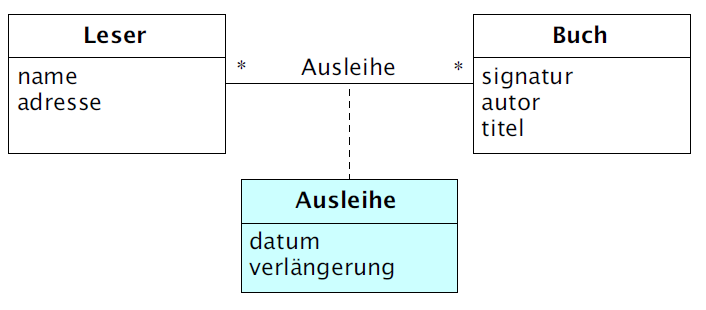
\includegraphics[width=6cm]{./bilder/Assoziationsklasse.png}}
    \parbox{6cm}{
      \item[Aggregation] 
        Sonderfall der Assoziation. "`ist Teilvon"' oder "`besteht aus"'.
      \item[Komposition] 
        starke Form der Aggregation. Beim löschen werden alle Teile gelöscht werden. 
        Jedes Teil kann nur zu einem Ganzen gehören}
    \parbox{9cm}{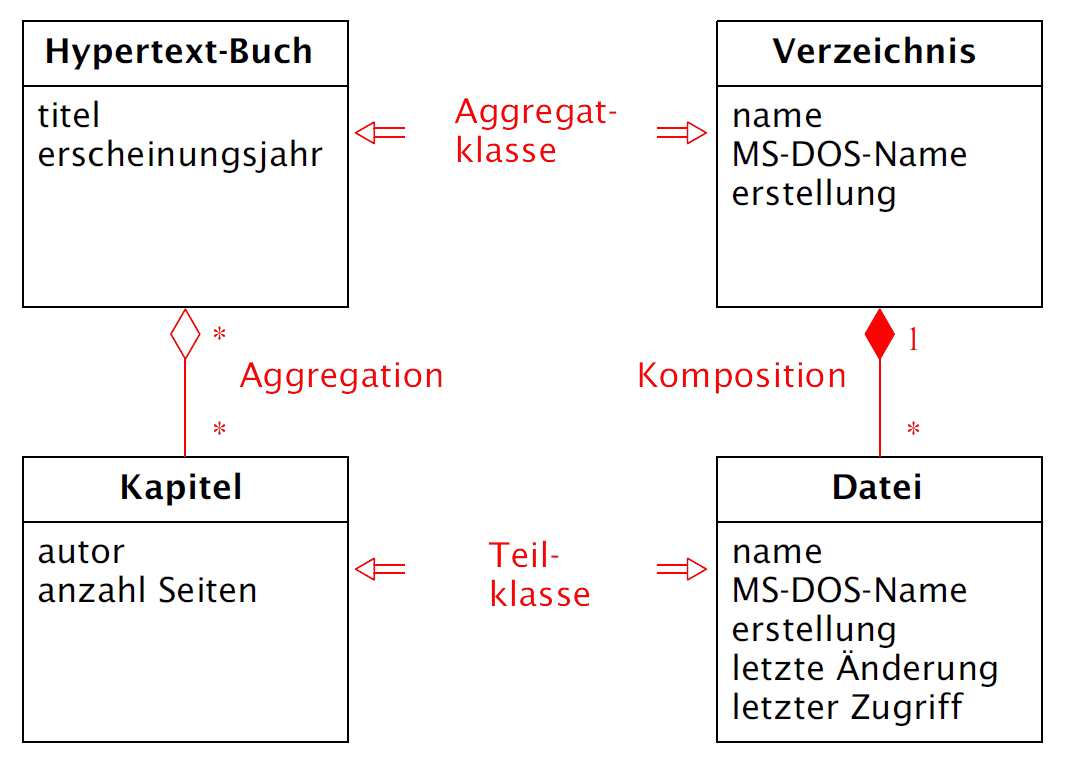
\includegraphics[width=6cm]{./bilder/Aggregation_Komposition.png}}
    \item[Multiplizität]
      \parbox{5cm}{Bezeichnet die Anzahl der an der Assoziation beteiligten Objekte.}
      \hspace{0.5cm}
      \parbox{4cm}{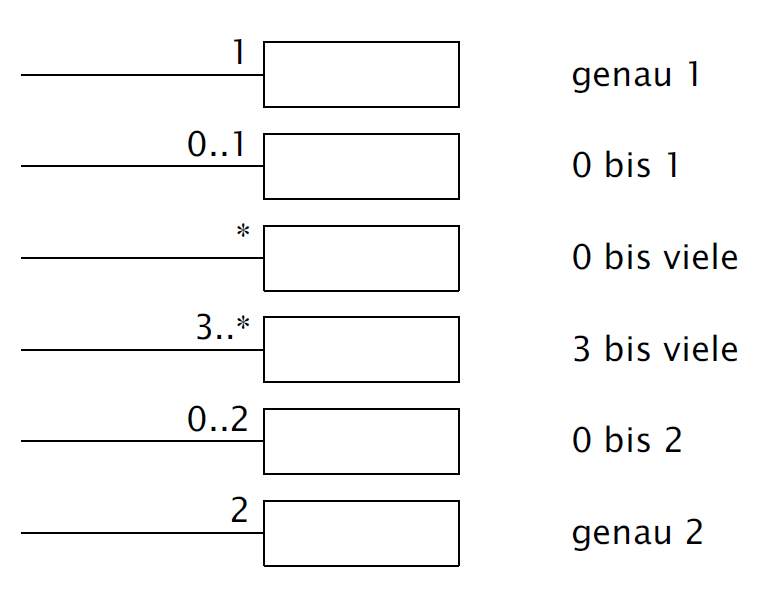
\includegraphics[width=4cm]{./bilder/Notation_Multiplizitaet.png}}
    \item[abgeleitete Assoziation] 
      Die Abhängigkeiten sind bereits durch andere Assoziationen beschrieben worden.
      Präfix "`\textbf{/}"'
    \item[Assoziationsname] 
      Beschreibt im Allgemeinen nur eine Richtung der Assoziation. 
    \item[Leserichtung] 
      Angabe beim Assoziationsnamen. Wird mit ausgefülltem, schwarzem Dreieck ($\RHD$) dargestellt.
    \item[Sichtbarkeit] 
      Vor dem Rollenname geschrieben. -private \#protected +public $\sim$package
    \item[Eigenschaftswert] 
      OOA: siehe \Balzert{45}
      
    \parbox{8cm}{
      \item[Rolle]
        Information oder die Bedeutung/Funktion einer Klasse in Beziehung zu einer anderen.
      \item[Rollenname]
        Jeweils am Ende der Assoziationsrichtung von der Klasse, 
        deren Bedeutung sie beschreibt. Kann zur Verständlichkeit beitragen. Ist zwingend für Reflexive Assoziationen.}
    \hspace{0.5cm}
    \parbox{6cm}{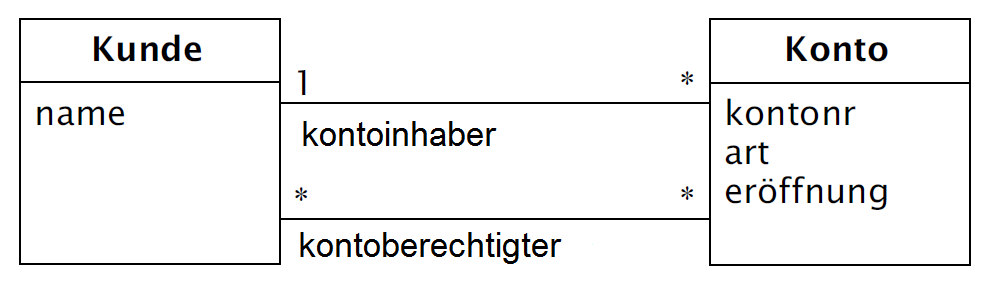
\includegraphics[width=6cm]{./bilder/Rolle.png}}
  \end{description}

\subsection{Generalisierung (Vererbung) \balzert{52}}
  Beschreibt die Beziehung zwischen einer allgemeinen Klasse (Basisklasse) und
  einer spezialisierten Klasse. Die spezialisierte Klasse ist vollständig
  konsistent mit der Basisklasse, enthält aber zusätzliche Informationen
  (Attribute, Operationen, Assoziationen). Jedes Objekt der Unterklasse \textbf{ist ein} 
  Objekt der Oberklasse.
   	
  \begin{description}
  	\parbox{8cm}{
    \item[Einfachvererbung]
      erbt von einer Basisklasse
    \item[Mehrfachvererbung]
      erbt von mehreren Basisklassen
    \item[Generalisierung] 
      Die spezialisierte Klasse erweitert die Liste der
      Attribute, Operationen und Assoziationen der Basisklasse
    \item[Generalisierungsmenge] 
      spezifiziert, nach welchen Kriterien eine Generalisierungsstruktur erstellt wird.
      (z.B. nach Tätigkeit, Job, etc.)}
  \parbox{9cm}{
  	\scalebox{1.3}{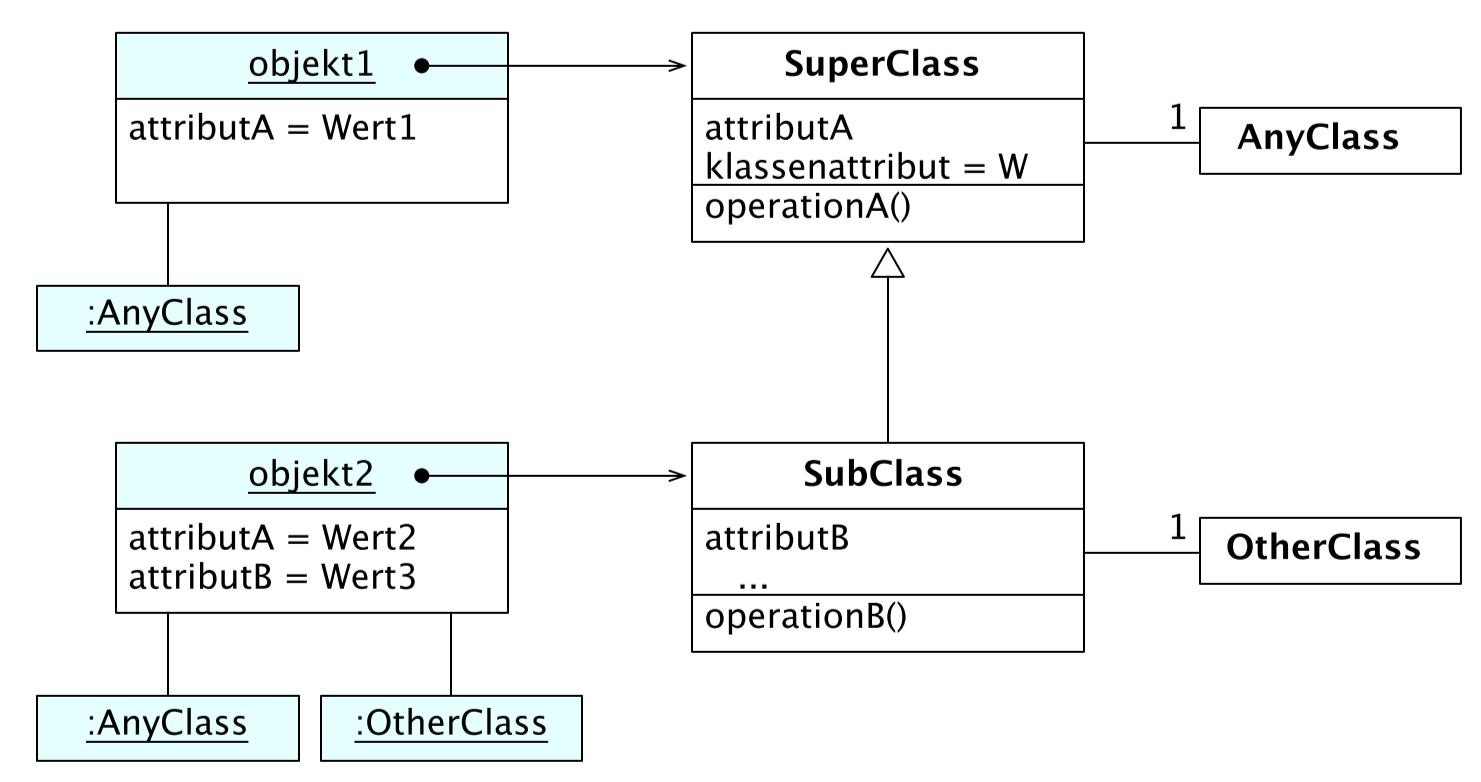
\includegraphics[width=5cm]{./bilder/Mechanismus_Vererbung}}
  }
  \end{description}

 \begin{multicols}{2}
	\subsection{Aktivität \balzert{69}}
  		Eine Aktivität beschreibt die Ausführung von Funktionalität bzw. Verhalten.

	\subsection{Zustandsautomat \balzert{87}}
 		 Zustandsdiagramm (finit state diagram)
 \end{multicols}
 
\subsection{Objektdiagramm (\textit{object diagram}) \balzert{21}}
	\begin{multicols}{2}
		Momentaufnahme / Schnappschuss des Systems. \\
		Beschreibt Objekte, Attributwerte, Objektbeziehungen zu einem bestimmten Zeitpunkt. \\
	\columnbreak
		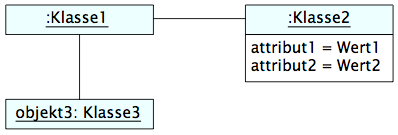
\includegraphics[width=5cm]{./bilder/objektdiagramm}
	\end{multicols}



\subsection{Use-Case Diagramm \balzert{62}}
	Ein Use-Case spezifiziert eine Sequenz von Aktionen
	\begin{description}[leftmargin=2.5cm]
		\item[Akteur]
      \parbox{7cm}{
        ist eine Rolle, die ein Benutzer des Systems spielt. Jeder Akteur hat einen 
        Einfluss auf das System. Befindet sich stets ausserhalb des Systems}
      \hspace{0.5cm}
      \parbox{6cm}{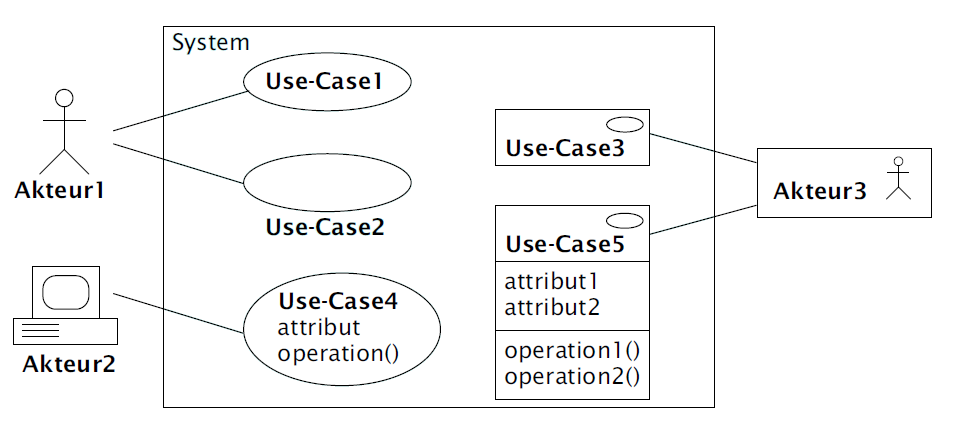
\includegraphics[width=6cm]{./bilder/UseCase_Notation.png}}
    \item[Schablone \Balzert{68}]
      \begin{itemize}[leftmargin=4cm]
        \item[\textit{Ziel:}]
          globale Zielsetzung bei erfolgreicher Ausführung des Geschäftsprozesses.
        \item[\textit{Kategroie:}]
          primär, sekundär, optional
        \item[\textit{Vorbedingung:}]
          erwarteter Zustand, bevor der Use-Case beginnt.
        \item[\textit{Nachbedingung Erfolg:}]
          erwarteter Zustand, nach erfolgreicher Ausführung des Use-Cases (Ergebnis)
        \item[\textit{Nachbedingung Fehlschlag:}]
          erwarteter Zustand, wenn das Ziel nicht erreicht werden kann
        \item[\textit{Akteure:}]
          Rollen von Personen oder anderen Systeme, die den Use-Case auslösen
          oder daran beteiligt sind.
        \item[\textit{Auslösendes Ereignis:}]
          Wenn dieses Ereignis eintritt, dann wird der Use-Case initiiert.
        \item[\textit{Beschreibung:}]
          \begin{enumerate}[leftmargin=0.5cm]
            \item Erste Aktion
            \item Zweite Aktion
          \end{enumerate}
        \item[\textit{Erweiterungen:}]
          \begin{enumerate}[leftmargin=0.5cm]
            \item[1a] Erweiterung des Funktionsumfangs der ersten Aktion
          \end{enumerate}
        \item[\textit{Alternativen:}]
          \begin{enumerate}[leftmargin=0.5cm]
            \item[1a] Alternative Ausführung der ersten Aktion
            \item[1b] Weitere Alternativen zur ersten Aktion
            \item[2b] ...
          \end{enumerate}
      \end{itemize}
	\end{description}

  %\begin{multicols}{2}
	\subsection{Szenario \balzert{80}}
  		Ein Szenario ist eine Sequenz von Verarbeitungsschritten, die unter bestimmten
  		Bedingungen auszuführen sind.\\
  		Die Szenarien lassen sich in zwei Kategorien unterteilen, die die eine erfolgreiche Bearbeitung
  des Use-Case beschreiben und jene Szenarien welche zu einem Fehlschlag führen. \\
  
  \textbf{Diagrammübersicht:}
  \begin{multicols}{2}
  	\begin{itemize}[leftmargin=0.5cm]
    	\item Sequenzdiagramm $\rightarrow$ \Balzert{81}
    	\item Kommunikationsdiagramm $\rightarrow$ \Balzert{85}
    	\item Timing-Diagramm
    	\item Interaktionsübersichtsdiagram
  	\end{itemize}
  \end{multicols}
  
\subsection{Analyseprozess \balzert{130}}
  Der Analyseprozess beschreibt die methodische Vorgehensweise zur Erstellung eines
  objektorientierten Analysemodells.\\
  
  Es besteht aus
  \begin{description}
    \item[Makroprozess]
      Der Makroprozess legt die methodischen Schritte fest, sprich in welcher
      Reihenfolge die Checklisten abgearbeitet werden $\rightarrow$ siehe \Balzert{132}
    \item[Checklisten]
      siehe \Balzert{133}
  \end{description}
  
  %\end{multicols}
  